\documentclass[twoside,a4]{report}
\def\atitle{Development of a Rheometer Controller Using a Raspberry Pi}
\def\shorttitle{Development of a Rheometer Controller}
\def\theauthor{Christopher Boyle}
\def\thewords{8514} % last proper build on Tue 21 March 2017 at 16:16:49
\def\br{\newline \newline \noindent}
\def\hi{\huge{!!!}}
\def\nohi{!!!! \normalsize}
\def\cbh{\large\bfseries !!! ??? !!! \normalsize\normalfont}

% Imports
\usepackage{graphicx}
\usepackage[a4paper]{geometry}
\usepackage{fancyhdr}
\usepackage[english]{babel}
\usepackage{etoolbox}
\usepackage{url}
\usepackage[hidelinks]{hyperref}
\usepackage{subcaption}
\usepackage[norefeq, prefix]{nomencl}

% Unused packages
%\usepackage{placeins}
%\usepackage{fancyref}
%\usepackage[comma,authoryear]{natbib}
%\usepackage{lipsum}

% Preamble
\makenomenclature
\renewcommand{\nomlabel}[1]{\hfil #1\hfil}
\nomenclature[a  a]{Symbol}{Description\hfill Units}


\geometry{top=2cm, bottom=2.5cm, left=3cm, right=2.5cm}  % Sets the mnargins
%\setcounter{secnumdepth}{0}  % removes the numbering from toc entires

\renewcommand\UrlFont{\rmfamily\itshape}  % sets URL font to normal font (rather than code font)

\setlength{\fboxsep}{0pt}  % separator length around figure boxes
\setlength{\fboxrule}{0pt}  % rule width around figures

\def\achapter{shorttitle}  % set the command "achapter" to  the name of the current section

\def\otherchap#1{
	\addtocounter{chapter}{1} 
	\def\achapter{\arabic{chapter} #1}
	\addcontentsline{toc}{chapter}{\achapter} 
	\chapter*{\achapter} 
	}

\def\rpilong{Raspberry Pi }
\def\rpi{Raspberry Pi }

%=====------++++++=====------++++++=====------++++++=====------++++++=====------++++++=====------++++++=====------++++++=====------++++++=====------++++++=====------++++++=====------++++++=====------++++++=====------++++++=====------++++++=====------++++++=====------++++++
% TEMPLATES

\iffalse  % This bit won't go onto the PDF


%%%EQUATION

	\begin{equation}
		(THE EQUATION)
		\label{EQUATION REF}
	\end{equation}


%%%FIGURE

	\begin{figure}[!htb]
		\centering
		\fbox{\includegraphics[scale=SCALE]{IMAGE LOCATION}}
		\caption{CAPTION}
		\label{FIGURE REF}
		%optional:
		\footnotesize [MORETEXT]
	\end{figure} \newline  \noindent

%%%BULLET POINT LIST
	\begin{itemize}
	\item
	\end{itemize}

\fi

%=====------++++++=====------++++++=====------++++++=====------++++++=====------++++++=====------++++++=====------++++++=====------++++++=====------++++++=====------++++++=====------++++++=====------++++++=====------++++++=====------++++++=====------++++++=====------++++++

% Header/footer preamble
\fancyhf{}  % clear the current header footer
\fancypagestyle{plain}{  % add settings for plain page style
	\renewcommand{\headrulewidth}{0.4pt}  % weight of the header rule (set to 0 for no line)
	\renewcommand{\footrulewidth}{0.4pt}  % height of the footer rule (set to 0 for no line)
%	\fancyhead[L]{\atitle}  % Header left is title
	\fancyhead[LE]{\achapter}  % Header left (even) is name of chapter
	\fancyhead[RO]{\shorttitle}  % Header right (odd) is report title
	\fancyhead[RE]{\theauthor}  % Header right (even) is author name
	\fancyhead[LO]{University of Strathclyde Chemical Engineering} % Header left (odd) is uni callout
	\fancyfoot[LO]{\today}  % Footer left (odd) is date
	\fancyfoot[RO,LE]{\thepage}  % Footer right (left on even) is page number
}
\pagestyle{plain}

\begin{document}
%% COPY HERE %%
%%%%%%%%%%%%%%%%%%%%%%%%%% TITLE PAGE
	\begin{titlepage}
		\makebox[\textwidth][c]{
\includegraphics[scale=1]{images/titleheader.png}}
		\centering
		\vskip3cm
		{
			\bfseries\Large
			Department of Chemical \& Process Engineering\\
			\vskip1cm
			MEng in Chemical \& Process Engineering\\
			18530
			\vskip3cm
			\LARGE\atitle
		}
		\vskip3cm
		{\small Word Count: \thewords}
		\vskip1cm
		\begin{flushleft}
			This project is submitted in partial fulfilment of the regulations governing the award of \\
			Degree of MEng in Chemical Engineering at the University of Strathclyde
			\vskip2cm
			Author: Christopher Boyle \hfill Date: \today \newline
			\vskip1cm
			Organisation: University of Strathclyde, Department of Chemical \& Process Engineering \newline
			%In-house Supervisor: Dr. Leo Lue \newline% \newline
			Academic Supervisor: Dr. Leo Lue
		\end{flushleft}
	\end{titlepage}

	%%%%%%%%%%%%%%%%%%% Main Content Settings
	\pagenumbering{roman}
	\setcounter{page}{0}
	\begin{center}\newpage \end{center}
	
	%%%%%%%%%%%%%%%%%%%%%%%%%%%%%%%%%%%%%%%%%% MAIN BODY PREAMBLE
	% Summary Page
	\otherchap{Summary} % last edited 14/3/2017
	%Brief, factual, generally following the same order of presentation as the report. Do not include figures, tables, or references.
	% WHAT WE DID
	A couette cell rotating rheometer was constructed, with the inner cylinder rotated by an electric motor. The rheometer was controlled by a Raspberry Pi computer using its GPIO ports to interact with electronic sensors and other hardware. \br
	% WHY WE DID IT
	The overall aim of the project was to design, build, and test a bespoke rheometer using a Raspberry Pi and open source software into order to create a device to help further our knowledge of the jamming phenomenon in colloidal suspensions.\br
	% HOW IT TURNED OUT
	The rheometer was evaluated by using it to measure the rheometry of various known solutions of water and glycerol. The rheometer's accuracy gauges by comparing the result with that from standard lab equipment. The rheometer [worked well/did not work well]. \cbh
	\newpage \begin{center} \large \space \normalsize \end{center}
	
	% Contents Page
	\newpage
	\def\achapter{Contents}
	\tableofcontents
	%\newpage \begin{center} \large \space \normalsize \end{center}
	% Acknowledgements
	\otherchap{Acknowledgements}
	%It is a matter of honesty and courtesy that acknowledgement is made to those who helped you in your work.
	First, I'd like to thank Dr. Leo Lue for his help and inspiration throughout this project. At every turn, he was there with new ideas and fresh ideas to keep me going. \br
	%Dr. Mark Haw - allowing the use of his research room
	I'd also like to thank Christopher Jones help with the lab equipment. Special thanks to Jim Murphy, who made the Couette cylinders himself. \br
	%Aditi Mukhopadhyay
	Finally, I'd like to thank the communities of the internet for telling me where I was going wrong, I would still be trying to spin a motor if not for them.
	
	\newpage
	\pagenumbering{arabic}
	\setcounter{page}{1}
	
%=====------++++++=====------++++++=====------++++++=====------++++++=====------++++++=====------++++++=====------++++++=====------++++++=====------++++++=====------++++++=====------++++++=====------++++++=====------++++++=====------++++++=====------++++++=====------++++++
                                                               
	\otherchap{Introduction} % section last edited 20/3/2017
	%The introduction sets the scene. It should include a brief description of the organisation, the type of work carried out, projects undertaken, background information to the work carried out and a brief outline of the report and of the learning objectives for the project.
	% Non-newtonian fluids exhibit interesting rheological properties: their viscosity can alter with shear stress (rheopectic) or time.\br
	Jamming is a special form of discontinuous shear thickening where a fluid experiencing shear appears to become solid. This causes problems in pharmaceuticals, food processing; industries where powders and suspensions are common. Jamming mainly causes transportation and mixing problems - situations where the fluid is sheared.\br
	This project aims to design, build, and test a control system for a bespoke rheometer (focused on recording the time variance of rheological properties). \br
	The hardware was controlled by a Raspberry Pi 3 Model B. The Raspberry Pi's low cost, low power consumption, and GPIO availability make it a suitable choice to control this process. Software was developed to take readings from sensors (giving the rotational speed and current supply) and record it. Further, software will be used to maintain a set rotational speed (or supply torque).\br
	Hardware was developed to allow the Raspberry Pi to obtain the most accurate readings from the experiment as possible; the rotational speed of the inner cylinder in the couette cell, and the current supplied to the motor. This information, along with the supply voltage, is used to calculate the viscosity of the fluid.\br
	[conclusion]


%=====------++++++=====------++++++=====------++++++=====------++++++=====------++++++=====------++++++=====------++++++=====------++++++=====------++++++=====------++++++=====------++++++=====------++++++=====------++++++=====------++++++=====------++++++=====------++++++


	\otherchap{Background} % section last edited 21/3/2017
	\section{Laboratory Automation and Process Control}
	Laboratory automation involves the design and implementation of robotic systems which are able to conduct laboratory experiments automatically, reducing the workload of human scientists and technicians \cite{backwhatisauto}. This includes the use of machine learning and AI to interpret results and create hypotheses \cite{backlitrevai, backbaconauto, backlabauto}. The motivation for this is eaasy to see, "Robot Scientists" can be used to conduct experiments with little to no human supervision and can take in a vast number of measurements. The "Adam" Robot Scientist developed by Aberystwyth University can make over a million observations and hypotheses per day \cite{backontorobsci}. 
	\br
	Laboratory automation emerged in the late 19th century, with siphons and controlled flow of water used to automate various processes. As technology advanced and electronics became more prevalent, the options for automation in the laboratory increased. Automatic titration equipment (using photo-cells to detect a colour change) were revolutionary in their ability to accurately and consistently record results, especially for difficult to discern colour changes \cite{backlabautohisto}. \br
	Process control can be thought of as the industrial mirror of laboratory automation which has developed along a similar path starting with mechanical analogue device, moving into electronically assisted technology and then, with the advent of computer technology, process control became the marriage of digital and analogue systems it is today \cite{backautocontrolhisto}.
	Process control is an inherent area of process design; the process (whatever it may be) has parameters which must be controlled so that the process continues under the design paramters; at the correct temperature, pressure, etc. Process control has historically been achieved through the use of analogue equipment, using pressurised air to send and receive signals from process equipment. Modern process control is achieved through the use of computers and digital electronics, where the analogue measured signals are converted into digital signals, so that a computer can understand the data. The controller applies an algorithm to calculate the control action required to maintain the desired value of the variable. The modern digital controller can deal with almost any form of input, guarding against a wide variety of disturbances. If it can be measured, it can be controlled.\br
	At the heart of the modern controller is the control algorithm. This is the calculation which determines what change to the control output needs to be made (the control action). Control algorithms vary with application. The most commonly used algorithm is the Proportional-Integral-Derivative algorithm (PID control), consisting of three sections which can be turned off or on depending on the needs of the situation:
	\begin{itemize}
		\item Proportional control increases the control action proportional to the size of the error (the difference between the set point and the measured value). This is easy to tune and set up, however it suffers from offset bias. This bias arise from the control action being balanced out in the process by the error such that the control action is not sufficient to change the process to compensate for the error. The error will remain, and the controller will do no more to correct for it, thus an offset is sustained. This must be manually corrected for.
		\item Integral control increases the control action depending on the integral of the error with respect to time (the longer the error goes on, the higher the control action). Integral action is useful to eliminate the offset bias of proportional control.
		\item Finally, derivative control increases control action with the derivative of the error with respect to time, so a quickly rising error is met with a large change in control action. Derivative action is difficult to tune and highly sensitive to noise in the circuit - this means it is rarely used. If it is used, it requires some form of noise filter on the signal and careful tuning. The most common version of the PID algorithm only uses proportional and integral action (no derivative) - the PI controller. PI control allows for easy tuning and quick response, without the difficulties of derivative action, or the offset bias of proportional control.
	\end{itemize}
	Each control element has an associated gain parameter which affects how strongly that element is represented in the control action. These parameters must be set properly before controller can be used. This is done in a process called tuning. There are a variety of methods for tuning the controller, most commonly used is the Ziegler-Nichols method, involving tuning the controller such that the measured value oscillates in a sustained way. Then using the period of oscillation along with other measured parameters to decide on the optimum controller tuning. After tuning using a method such as Ziegler-Nichols it is often required to tweak the tuning manually to obtain the most effective controller for the situation. This is done mostly by trial and error. Trial and error tuning can also be used to fully tune the device, although this would take a long time to do by hand. \br
	The controller device itself is a small computer, reading input from the instruments and then applying the algorithm to determine how it should alter the process. These small computers are called "microcontrollers". A microcontroller chip is a small re-programmable computer which reads input from, and outputs data to an electronic circuit \cite{backwhatismc}. Microcontrollers are programmed by connecting them to a "master" computer which can set the data on the microcontroller's storage. Data is stored as binary data (data is stored solely in the form of 0s and 1s). The program is written in a programming language, a special set of instructions which the environment can understand and convert into actions. \br
	
	\section{Raspberry Pi} % section last edited 3/3/2017
	\noindent
	Microcontrollers are commonly used in education to teach computer programming \cite{backmcedu1, backmcedu2}. However, it was noticed that people were not properly learning about how computers work in schools and universities and so a team of academics at the University of Cambridge created the Raspberry Pi Foundation, and developed the Raspberry Pi Model A as a platform to facilitate education \cite{pihistory}. The Raspberry Pi is a small (85mm x 56mm \cite{pi3mechdraw}) computer. By default, it runs a version of GNU/Linux called "Raspian". There are a number of alternative operating systems suitable for different applications (media center, embedded smart technology) \cite{piotheros}.  \newline
	\begin{figure}[!htb]
		\centering
		\fbox{\includegraphics[scale=0.3]{images/annotpidia.png}} %https://www.draw.io/#Hcbosoft%2Fpi_rheo_proj%2Fmaster%2Fwrite_up%2Fimages%2Fannot_pi_dia.xml
		\caption{Raspberry Pi 3 Model B (adapted from  \cite{pi3info})}
		\label{pidia}
	\end{figure} \newline% \noindent
	The first Raspberry Pi (Model A) had a single core 700MHz processor and 256MB of RAM \cite{pi1info}, while the current Raspberry Pi 3 Model B has a quad core 1.2GHz and 1GB of RAM (also including built in WiFi and Bluetooth) \cite{pi3info}. The quad core processor enables better multi-threaded operation for software running on the Raspberry Pi, meaning that big cumbersome programs can run much more efficiently than before. In addition, the increase in memory and CPU clock frequency means there is overall a massive performance boost. Operations like compiling a large program (for example OpenCV, the Open Source Computer Vision Library) which could take over 9 hours \cite{pipowercompold} on the Raspberry Pi 1, takes little over an hour and a half \cite{pipowercompnew} on the latest model.\br
	Despite being initially designed for educational purposes, the Raspberry Pi has found success in other areas such as with hobbyists \cite{pihobbynotedu} and in industry \cite{pimorethanedu}. What makes the Raspberry Pi attractive as a process controller are the GPIO pins (General Purpose Input/Output, see Figure \ref{pidia}) made available on the main board, similar to a microcontroller. These pins allow electronic circuits to interface with the Raspberry Pi, and thus software to interact with the real world in a way that is not easy to accomplish with a traditional computer. This marriage of microcontroller and desktop computer allows for development, and testing in a single package. In addition, the Raspberry Pi retails (at the time of writing) for \pounds 30.00 \cite{picost}, making it a very cost effective alternative to other control solutions (which can cost several hundred pounds \cite{otherpcucost}). \br
	The GPIO pins are the heart of the Raspberry Pi. Each pin is numbered so that they can be referenced and distinguished between their functions. Some of the pins on the GPIO header are power pins (e.g.  pins 1,2 and 4), some are ground (e.g. 6, 9, and 14), and most are GPIO pins (e.g. 3, 5, and 7). Each GPIO pin can be either low or high. This can be set in different ways; resistors attached to the GPIO pins can be used to "pull-up" or "pull-down" the signal. If a pin is pulled down, its signal is normally low - it needs to be actively raised high. If a signal is pulled up, it is normally high - it can be lowered by connecting it to ground, but without that it will try to be high. These pull-up and pull-down resistors are included in the Raspberry Pi internally and can be turned on or off via software. \newline
	\begin{figure}[!htb]
		\centering
		\fbox{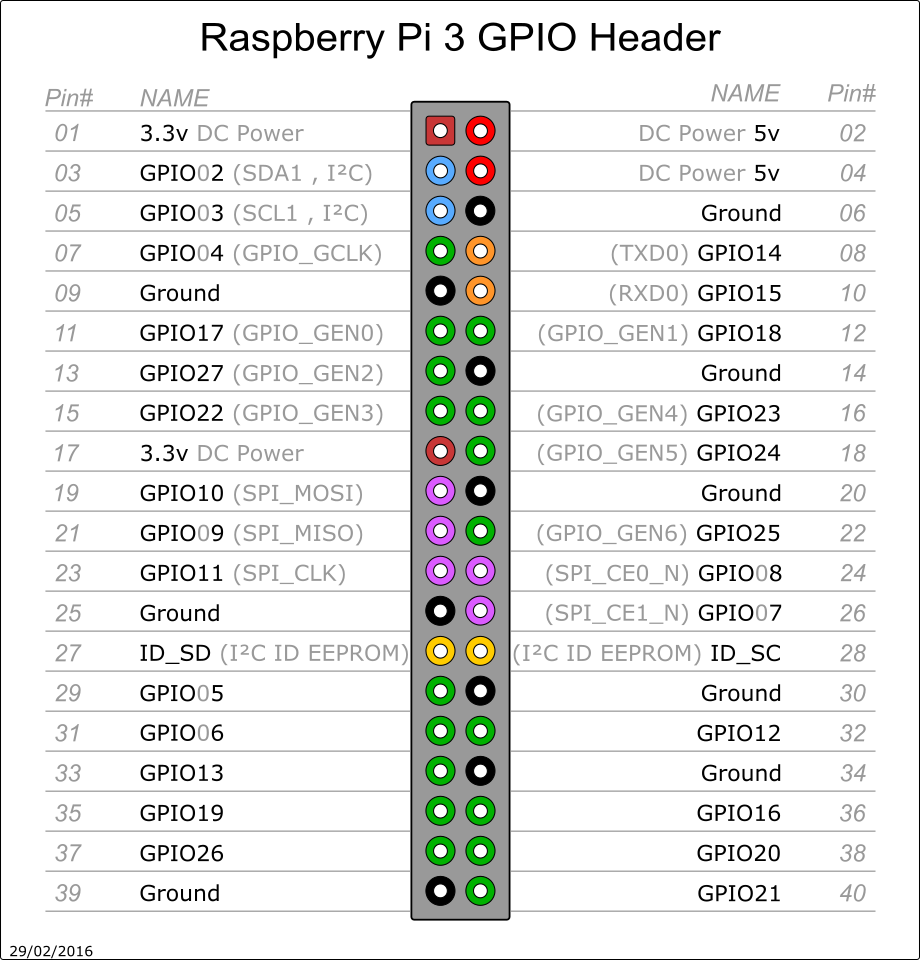
\includegraphics[scale=0.2]{images/gpiopinout.png}}
		\caption{Raspberry Pi 3 Model B GPIO Pinout Diagram (taken from  \cite{pigpiopinout})}
		\label{gpiopinout}
	\end{figure} \newline  \noindent
	In addition to simple GPIO functionality, some of the Raspberry Pi's GPIO pins have special functionality, like the ability to use serial communication making inter-device communication much easier. To send the number 1750 to an integrated circuit, the Raspberry Pi would need at least 11 free GPIO pins. While this is not impossible, the number of GPIO pins taken up by the single device is extremely inconvenient. This can easily be sent via serial connection with just two wires. Pins 3 and 5 can also be used to communicate with integrated circuits with the \(I^2 C\) protocol (Inter-Integrated Circuit). This allows bytes of data to be sent over only two wires \cite{backwhatisi2c}. This is done by \textit{serial communication}. Serial communication is where each bit of data (starting with the most significant bit, the highest value bit) is sent one after the other down a wire (the "data" line) \cite{backwhatisserpar} while another wire is used to synchronise the communication beteween devices (the "clock" line). Pins 19, 21, 23, 24, and 26 are used for another serial communications protocol, the Serial Peripherial Interface (SPI) protocol \cite{backwhatisspi}. SPI is similar to \(I^2 C\), although it differs in a few key ways.  \(I^2 C\) manages sub devices on the network using an address system which enables anything up to 128 devices connected together in one go, however SPI uses a simple select system where a signal is sent from a GPIO to the SPI device to tell it to expect instruction. This makes the SPI device far easier to work with, but less useful as the number of daisy-chained devices is limited by the number of free GPIO pins. \br
	The high level languages used to create programs on desktop computers can be similarly used to write software on the Raspberry Pi. There are a number of software packages available for facilitating the communication with the GPIO pins. Built in to the Raspberry Pi are some basic packages, but for greater functionality third-party libraries are available for anyone to download and use\cite{pilibswiringpi, pilibspigpio}. The programming language "Python" is popular among software developers. Python is a high level, object oriented, interpreted language; making it well suited to quickly develop clean and easy to use software. Due to its popularity, Python has a vast number of packages available to perform any number of functions.
	
	\section{Rheometry} % last edited 8/3/2017
	The viscosity of a fluid is a measure of how resistant it is to flow. This is an important concept in process engineering: most processes involve fluids, many products are have fluid components. The viscosity (\(\mu\)) of a fluid can be calculated from the shear stress (\(\tau\)) imposed on a fluid and the rate at which it shears(\(\dot{\gamma}\)) using Newton's Law of Viscosity (Equation \ref{eqnvisco}) \cite{backfluidmech}.
	\begin{equation}
	\mu = \frac{\tau}{\dot{\gamma}}
	\label{eqnvisco}
	\end{equation}
	There are different classes of fluids depending on how their viscosity behaves with respect to shear rate (the speed of the deformation) or the shear stress (the force behind the deformation). Newtonian fluids (like water) have a viscosity which is independent of the shear stress - proportional only to the shear rate. Some fluids have time-dependant viscosities: thixotropic fluids have a viscosity which apparently reduces the longer a stress is applied, and rheopectic fluids have a viscosity which apparently increases the longer a stress is applied. Other non-Newtonian fluids are dependant on the magnitude of the stress: shear-thinning fluids have a viscosity that appears to decrease with increased stress, and shear thickening fluids appear to experience a viscosity increase with an increase in stress \cite{backtypesofnonnewt}. Figures \ref{figshearthin} \& \ref{figshearthick} give examples of how shear rate varies with shear stress for non-Newtonian fluids. \br
	\begin{figure}[!htb]
		\centering
		\fbox{
			\begin{subfigure}[t]{0.45\textwidth}
				\centering
				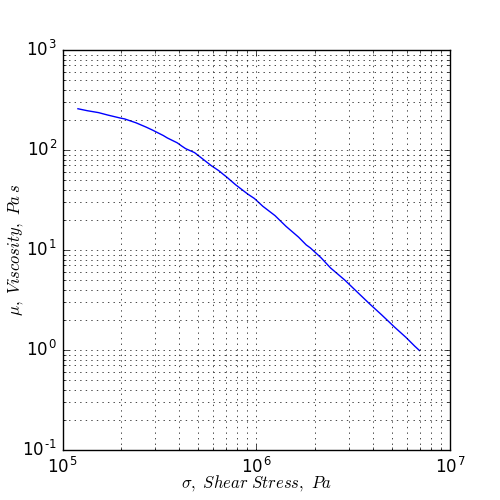
\includegraphics[scale=0.5]{figures/fig_shear_behav_thin.png}
				\caption{Shear Thinning}
				\label{figshearthin}
			\end{subfigure}
			\begin{subfigure}[t]{0.45\textwidth}
				\centering
				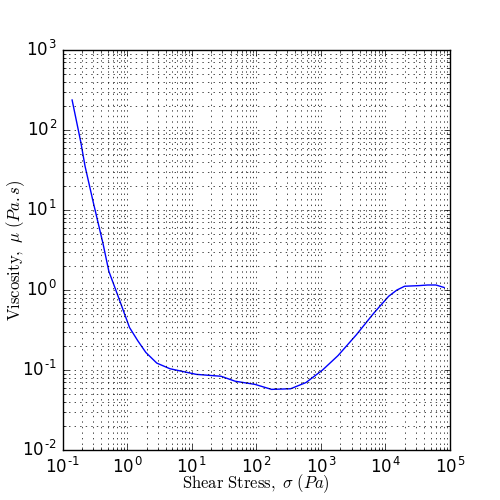
\includegraphics[scale=0.5]{figures/fig_shear_behav_thick.png}
				\caption{Shear Thickening}
				\label{figshearthick}
			\end{subfigure}
			%\fbox{\includegraphics[scale=0.25]{figures/fig_shear_behav.png}}
		}
		\label{figshearthinthick}
		\caption{Non-Newtonian Behaviour: Viscosity vs Shear Stress (adapted from \cite{figshearthin, figshearthick})}
	\end{figure} %\newline  \noindent
	Viscosity is measured in the lab using a rheometer. There are several distinct types of rheometers: capillary rheometers flow the fluid through a pipe of known dimensions and use the time taken to calculate the viscosity, cone-and-plate rheomters use a plate upon which is the fluid to be tested, and into the fluid is placed a cone which is spun (using the geometry and the torque/rotational rate of the spinning cone to calulate the viscosity), and the rotational rheometer which consists of a cylinder within another with the fluid to be tested between the cylinders such that it shears when a cylinder is rotated. \br
	The capillary rheometer consists of a tube of known cross section, through which the test fluid is forced (by pumping, by piston). The viscosity can be found by measuring the flow rate and pressure gradient, and using the Hagen-Poiseulle equation for laminar flow through a pipe \cite{backcaprheom}.\br
	The cone-and-plate rheometer \cbh \br %(Information about the CAPR: how does it work, how accurate can it be, what is it usually used for)
	The rotational rheometer is based upon the idea of couette flow: two infinitely long plates (separated by a known amount) between which is the fluid. In this scenario, \cbh
	constructed from two cylinders: the outer (hollow) cylinder and the inner cylinder. The cylinders are positioned vertically close together to limit the amount of fluid shearing on the bottom of the inner cylinder.
	
	\section{Colloidal Suspensions and Jamming} % last edited 8/3/2017
	Fluids consisting of solid particles suspended in a liquid are prone to non-Newtonian behaviour, most commonly shear thinning (pseudoplastic). Some suspensions exhibit shear thickening behaviour, which has been explained in a number of ways. One theory explaining the onset of DST is the hydroclustering theory: as the suspension undergoes shear, the particles are forced together, forming larger particle groups. This increases the effective viscosity compared to low shear flow where the particles movements are not as restricted \cite[p.~7]{backbrownjaegrev}.
	The order-disorder transition  theory explains the increase in viscosity as being due to an increase in stress causing the particles to become disordered. Initially there is a drop in viscosity, due to the particles in the suspension becoming more ordered. Then, as the stress is increased past a yield stress, the viscosity begins to increase due to a disruption in the order of the particles. % other theories?
	\cbh \br
	Shear thickening can be split further into continuous shear thickening (CST) and discontinuous shear thickening (DST, also termed dilatancy). CST is where the viscosity increases proportionally past a yield stress. However, with DST the viscosity suddenly (almost asymptotically) jumps upwards after a yield stress. DST has been associated with an apparent decrease in volume fraction of suspensions - hence its alternative name of dilatency. This effect also lends credence to the order-disorder-transition theory of shear thickening: you would expect the volume fraction to decrease (void fraction to increase) if the particles are going from a neat, ordered arrangement into extreme disorder \cite[p.~7]{backbrownjaegrev}. \cbh \br % cite!
	DST is thought to be closely linked to the concept of jamming, which is \textit{"the conversion of a liquid system into a solid by imposed stress"} \cite{backhawjam}. Jamming is found in many different systems: in solids entering a hopper \cite{back2djam}, in pedestrians walking down a corridor \cite{backpedjam}, and in traffic \cite{backcarjam}. This can cause problems in processes: halting flow, damaging mixing equipment \cite{backshearjambertrand}. \br 
	Volume fraction of the suspension mixture is an important property when looking at jamming. A suspension's volume fraction (\( \Phi \)) is the ratio of the volume of suspended particles to the volume of fluid in the suspension. For spherical particles, there is a maximum fraction. The closest packing that can occur (face-centred cubic) results in a particle volume fraction of \( \Phi = 0.74 \). However, at this packing the suspension is no longer a suspension and the particles are all in constant contact. The highest volume fraction of a suspension that still allows fluid to pass between the particles (particles are lubricated) is \( \Phi = 0.64 \) \cite{backguypoonjam}. As volume fraction increases, the likelihood of a suspension to undergo jamming increases (CITE). \br
	Hard spheres is an approximation of the physical properties of the particles in a suspension. A "hard sphere" particle is a particle which is roughly spherical and with a fixed (non-intersectable) volume. \cbh \br
	% "Normal" fluids (like water) exhibit Newtonian behaviour, this means that the rate of shear (how fast they deform) is directly proportional to the shear stress imposed upon them, with the constant of proportionality being the viscosity of the fluid\cite[p.~252]{schadict}. Multiphase suspensions can exhibit non-Newtonian viscous behaviour, where this direct relationship is not found \cite[p.~255-256]{schadict}. Some exhibit a shear-thickening behaviour: as the shear stress is increased, the shear rate decreases faster than in newtonian behaviour and others exhibit shear thinning .  Continuous shear thickening (shown in Figure \ref{figshearthick})  is an increase in the apparent viscosity. Discontinuous shear thickening is a sudden and extreme increase in the apparent viscosity of the fluid and is closely related to jamming, which is \textit{"the conversion of a liquid system into a solid by imposed stress"} \cite{backhawjam}. Jamming is found in many different systems: in solids entering a hopper \cite{back2djam}, in pedestrians walking down a corridor \cite{backpedjam}, and in traffic \cite{backcarjam}. This can cause problems in processes: halting flow, damaging mixing equipment \cite{backshearjambertrand}. \br	
	%flow, shear, jam frequency %TODO
	An interesting phenomenon that occurs in shearing suspensions is the formation and dissipation of "cracks" on the surface of the suspension. This can be directly seen in Figure \ref{cforscracks}. The cracks have been associated with a localized change in volume faction of the suspended particles \cite{backhawjam}. Another interesting optical property of jammed suspensions: the surface of a shear suspension has been found to alter texture, evidence of "Dilation" \cite{backbrownjaegrev}: caused by the particles in shear attempting to move around each other but having to take an inefficient route therefore decreasing the volume fraction of the suspension. This draws more fluid into the bulk and then the surface appears rough in texture, as opposed to glossy. 
	\newline \newline \noindent
	\begin{figure}[!htb]
		\centering
		\fbox{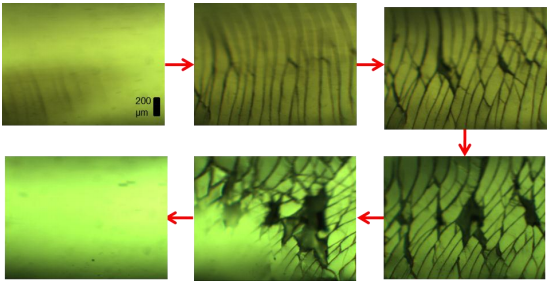
\includegraphics[scale=0.4]{images/cfors_cracks.png}}
		\caption{Suspension Surface Cracks (taken from \cite[p.~118]{thescforsyth})}
		\label{cforscracks}
	\end{figure} \newline  \noindent


%=====------++++++=====------++++++=====------++++++=====------++++++=====------++++++=====------++++++=====------++++++=====------++++++=====------++++++=====------++++++=====------++++++=====------++++++=====------++++++=====------++++++=====------++++++=====------++++++

	\otherchap{Description of the Work}
	%Elaborate on issues mentioned in introduction. Use a logical development, not necessarily in chronological order. Explain the significance, purpose and nature of your work. Describe methods used and outcomes. Try to ensure a balanced treatment of issues, in accordance with their relative importance, and excluding irrelevant material. Present results and discuss around them. Explain the significance of these results and their impact on the organisation. Comment on technical difficulties you may have experienced. In a long report, subdivide with appropriate sub-headings, or divide this section into different sections. Equations should be numbered sequentially.



	\section{Hardware Setup} % last edited 7/3/2017
	The experiment is based around a Couette cell (CITE), consisting of two concentric cylinders with a fluid in between. The inner cylinder can be rotated by a DC motor (SERNO) while the outer cylinder is fixed. The motor is controlled by a raspberry pi, which sets its speed and reads in the torque load on the motor. This is used to calculate the viscosity of the fluid. 
	Motor speed is read in using a secondary motor acting as a dynamo. This dynamo is spun by the inner cylinder motor and produces a voltage proportional to its rotational speed. This voltage is then read in by the \rpi.
	A needle attached to a piezo-electric (termed the Piezo-Electric Needle Device or PEND) is used to detect shear stress at a point within the fluid. When the fluid jams, the needle will move and generate a voltage proportional to the needle's displacement. Figure \ref{expdia} gives a diagram of the set-up.\newline
	\begin{figure}[!htb]
	\centering
	\fbox{\includegraphics[scale=0.3]{images/exp_set_up.png}} % https://www.draw.io/#Hcbosoft%2Fpi_rheo_proj%2Fmaster%2Fwrite_up%2Fimages%2Fexp_set_up.xml
	\caption{Diagram of the Experimental Apparatus}
	\label{expdia}
	\end{figure} \newline \noindent
	% TODO :: UNCERTAINTIES IN MEASUREMENTS, MEASUREMENTS
	The outer cylinder is a hollow glass cylinder, closed at one end. It has an outer diameter of 44.151mm, and inner diameter of 39.111mm, a height of 39.753mm. The cylinder has been glued to a metal plate which holds it in place. \br
	The inner cylinder is a perspex cylinder built onto the motor's shaft. The cylinder is 30.215mm in diameter and 46.795mm in height. There is a thinner section of the cylinder at the top of the main cylinder, which is used as a pulley for the belt to hold on to (see Figure \ref{expdia}). \br
	The motor, holding the inner cylinder, is held in place by a clamp stand. This clamp stand also holds the dynamo in position.\br
	The electronic circuits were built onto breadboards. This allowed for simple and quick alterations to be made to the circuitry during development. Wires connect the electronics to the motor, dynamo, and the power source. A ribbon cable connects the full 40 GPIO pins from the raspberry pi to the breadboard circuitry.
	
	\section{Electronic Circuits} % last edited 7/3/2017
	%in depth description of relevant electronic circuits
	The electronic circuits attached to the Raspberry Pi can be split into two distinct sections. The motor speed detection circuit converts the rotational speed of the motor to a digital signal, and the motor speed control converts a digital signal into rotation of the motor. See Figure \ref{circfull} for an overall diagram of the circuit.
	\begin{figure}[!htb]
		\centering
		\fbox{\includegraphics[scale=0.3]{images/circfull.png}}
		%https://www.draw.io/#Hcbosoft%2Fpi_rheo_proj%2Fmaster%2Fwrite_up%2Fimages%2Fcircfull.xml
		\caption{Schematic Diagram of Electronic Circuits}
		\label{circfull}
	\end{figure}
	\cbh %diagram is missing SPI links

	\subsection*{\textit{Motor Speed Detection}} % last edited 13/3/2017
	%Dynamo
	The speed of the motor was gauged using a second motor acting as a dynamo. The dynamo motor was linked to the first motor by a belt and pulley system. The dynamo motor produces a voltage proportional to the speed it is spun at. This voltage was amplified using an operational amplifier circuit by a factor of ten and read in using an ADC (MCP3008). This was calibrated by setting the potentiometer to different values and recording the voltage produced by the dynamo. Then the speed at these known potentiometer values was found using a tachometer (SERNO). Thus the speed as a function of the dynamo voltage can be calculated. \br
	There is also a provision for being able to detect the current supplied to the motor. This is achieved using a Hall Effect sensor and inductor package (ACS712). This uses a Hall Effect sensor to detect the size of the magnetic field generated by the current passing through an inductor, producing a voltage proportional to the magnitude of the current. This signal is passed through an op-amp (LM358) to bring it up to a suitable level for the ADC to read.
	

	\subsection*{\textit{Motor Speed Control}} % last edited 7/3/2017
	%Nomenclature in this section:
	The speed of the motor is sent from the Raspberry Pi as a digital serial signal (using the SPI protocol) to a digital potentiometer (MCP4131), a device which can electronically adjust the resistance between its pins. Within the potentiometer:\(R_{AW}\) is the resistance between terminal Aand the wiper pin, and \(R_{WB}\) is the resistance between the wiper and terminal B. The data sent to the potentiometer determines the values of \(R_{AW}\) and \(R_{WB}\), which will total a constant value: \(R_{pot} = 10\ k\Omega \). The digital potentiometer is used in a voltage divider configuration, which allows the voltage in a parallel circuit to be controlled. When the resistance is changed to a new value, the voltage across the motor will change according to Equation \ref{eqnvoldiv}. Resistor \(R_2\) is used to set the minimum output voltage. At \(R_2 = 0\ \Omega\), the output would vary between 0v and 5v. While this would also be useful, it limits the resolution of the potentiometer as teh bottom volt of this range will not be able to sufficiently power the motor. To bring this minimum up (and thus be able to utilise more of the potentiometer) \(R_2\) is set at \(3\ k\Omega \). The digital potentiometer can only handle voltages up to 5v across its terminals, an amplifier (gain = 2.1) is used to boost the voltage range from 1.2v to 5v up to 2.52v to 10.5v. A transistor (BD243C) is used to boost the current output from the amplifier, which can only supply around 20mA. The Transistor boosts this up to 2A (assuming a conservative gain of hFE = 100).
	\begin{equation}
		V_{out} = V_{in}\times \frac{R_2 + R_{WB}}{R_2 + R_{pot}}
		\label{eqnvoldiv}
	\end{equation}
	\begin{equation}
		V_{min} = V_{in}\times \frac{R_2}{R_2 + R_{pot}}
		\label{eqnminvol}
	\end{equation}
	\begin{equation}
		V_{max} = V_{in}\times \frac{R_2 + R_{pot}}{R_2 + R_{pot}} = V_{in}
		\label{eqnmaxvol}
	\end{equation}
	
	\nomenclature[aV ]{$V_{out}$}{Voltage output \hfill $V$}
	\nomenclature[aV ]{$V_{in}$}{Voltage input \hfill $V$}
	\nomenclature{$R_{AW}$}{Resistance between potentiometer wiper and A terminal\hfill $\Omega$}
	\nomenclature{$R_{WB}$}{Resistance between potentiometer terminal B and wiper\hfill $\Omega$}
	\nomenclature{$R_{pot}$}{Resistance between terminals A and B on the potentiometer\hfill $\Omega$}
	\nomenclature{$R_{AW}$}{Resistance value ofthe resistor between B terminal on the potentiometer and ground\hfill $\Omega$}
	
	\noindent
	The Raspberry Pi sets the motor speed by setting the resistance in the digital potentiometer. The Pi sends a 7-bit digital signal to the pot, indicating the resistance desired. Within the potentiometer is a network of resistors, and this number will determine the path the circuit takes through the circuit, the higher the number, the higher the resistance between the A terminal and the wiper, \(R_{AW}\). When this increases, the voltage across the bottom resistor will decrease and the voltage across the motor will mirror this.\br
	The 7-bit has 128 possible configurations ($2^7 = 128$). Therefore the potentiometer terminal B-wiper resistance will increase by $78 \Omega$ given a unit increment in potentiometer value (Equation \ref{eqnpotres}). Combining this with Equation \ref{eqnvoldiv} gives an equation for motor supply voltage (also knowing the gain of the operational amplifier circuit) - Equation \ref{eqnmotsupvol}.
	
	\begin{equation}
	V_{wiper} = V_{AB}\times \frac{3k\Omega + \left(78\Omega \times pv\right)}{13k\Omega}
	\label{eqnpotres}
	\end{equation}
	
	\nomenclature[aV ]{$V_{wiper}$}{Voltage level at the digital potentiometer output \hfill $V$}
	\nomenclature[aV ]{$V_{AB}$}{Voltage accross the potentiometer terminals\hfill $V$}
	
	\begin{equation}
	V_{ms} = 0.0631 \times pv + 2.423
	\label{eqnmotsupvol}
	\end{equation}
	
	\nomenclature[aV ]{$V_{ms}$}{Motor supply voltage\hfill $V$}
	%Similarly, when \(R_{AW}\) decreases, the voltage in the bottom half of the divider will increase and so will the voltage across the motor. The resistors included in addition to the digital potentiometer set the minimum and maximum values for the voltage across the motor, the minimum voltage is where the wiper resistance is essentially zero, so Equation \ref{eqnvoldiv} becomes Equation \ref{eqnminvol}. For maximum voltage, the wiper is set as high as possible (\(R_{WB} = R_{pot}\)) and Equation \ref{eqnvoldiv} becomes Equation \ref{eqnmaxvol}. 
	%\subsection{\textit{PEND Input Processing}}

	\section{Software} % last edited 13/3/2017 %uml?
	Software was written to enable the \rpi to communicate with the hardware. The Python language was chosen as it is a very popular, easy to use, and easy to read language. Its popularity means that there is a swathe of software packages available for inclusion. These packages contain pre-written code, meaning that something that has already been done (and done well) does not have to be written again - representing a significant time saving due to not having to debug a whole section of code.\br
	The hardware designed for this project makes heavy use of the SPI protocol - a kind of serial communication. The SPI protocol can be accessed in a python environment by using the \texttt{spidev} package \cite{srcspidev}. This package makes functions available to create a connection to an SPI device, to send data, and to receive data. This package is used to set the resistance on the digital potentiometer, and to read signal information from the analogue to digital converter. \br
	The software is organised into different classes:
	\begin{itemize}
		\item Digital Potentiometer \newline 
		This class manages the sending of data to a digital potentiometer and keeps a record of some key data.
		\item ADC \newline 
		This class manages the sending and receiving of data between the \rpi and an ADC.
		\item Control\newline 
		This class is a discrete time implementation of the PID algorithm used in process control.
		\item Motor \newline
		This class makes use of the digital potentiometer class to control the voltage supplied to the motor, the ADC class to read in the speed of the motor and the current drawn by the motor. This data is logged at a set rate to be used in calculating the viscosity.
		\item Noise Filter \newline
		Not a class, but a collection of functions that can be used to reduce noise in read data.
	\end{itemize}
	Full copies of the software source code can be found in Appendix 1.
	
	%Section detail
	\subsection*{Digital Potentiometer} % last edited 13/3/2017
	% Description
	This class enables the software to interact with the digital potentiometer (model MCP4131) using the SPI protocol. This class makes use of the spidev package to enable SPI communication. The class contains a function to set a value on the resistor (as an integer number between 0 and 127), and is set up such that multiple digital potentiometers can be included on the same circuit.\br
	% Usage
	The class is used, as with all normal classes, by first creating an instance of a class object, passing along the initialisation parameters. These parameters are set in the source code as the parameters to the "\texttt{\_\_init\_\_}" function. For this class, there is only one initialisation parameter: "\texttt{chip\_select}", an optional parameter which tells the spidev package which SPI device to talk to. This parameter is 0 by default, but can be changed if the class is used in a different instance to manage another digital potentiometer.\br
	To set the resistance on the potentiometer, a value between 0 and 127 (inclusive) is sent to the potentiometer using the "\texttt{set\_resistance}" function. This function only requires one parameter - the value to be sent. Then it uses the spidev package to send this value to the correct register on the potentiometer, causing it to alter its resistance.
	%What else to include?
	
	\subsection*{ADC} % last edited 13/3/2017
	The ADC class enables the software to interact with the analogue to digital converter (both model MCP3008) via the SPI protocol. As with the digital potentiometer, this class makes use of the spidev package. Again, just as before, multiple instances can be used in conjunction to manage reading data from different ADCs connected to the \rpi at the same time. \br
	The initialisation function for the ADC class has two parameters, both optional. The first is a chip select parameter (used to tell spidev which device we are trying to communicate with on the SPI network) which has a value of 1 by default. The second parameter is the value of the reference voltage (\texttt{vref}), 3.3 by default, used to calculate the voltage read in by the ADC from the 10-bit value read from the ADC. \br
	Usage of the class is very simple: the "\texttt{read\_data}" function returns the value read from the ADC (a 10-bit number) and takes only 1 parameter (a value from 0 to 7 indicating the channel on the ADC to read from). Further, the "\texttt{read\_volts}" function will read from the ADC and convert the result to a voltage. This function takes a channel indication parameter.
	
	\subsection*{Control} % last edited 13/3/2017
	This class is primarily a discrete-time implementation of the PID algorithm, also known as the velocity algorithm (Equation \ref{eqdiscpid}).\br
	The initialisation function for this class accepts five optional arguments:
	\begin{itemize}
		\item KP, the proportional control coefficient. 0 by default.
		\item KI, the integral control coefficient. 0 by default.
		\item KD, the derivative control coefficient. 0 by default.
		\item sample\_time, the interval time between control action updates. By default, this is automatically calculated, but can be set manually here for simulating the response.
		\item set\_point, what is the desired value for the controlled process variable. 0 by default.
	\end{itemize}
	For the PID controller to be useful, it needs to be tuned. This can be done using a model transfer of the process and the "\texttt{tune}" function. This function will iterate through a range of possible tunings and decide upon the best solution based upon the model's response to a step change in set point. This decision is based upon rise time, and stability (amount of response oscillation). Alternatively, the tune function will based the optimal tuning upon the integral-squared-error (ISE) value of the result. The model must be first order, its parameters (time constant "\texttt{time\_constant}" and steady state gain "\texttt{steady\_state\_gain}") are passed to the tune function as required arguments. Optional arguments are the ranges for the tuning to iterate through for each tuning parameter: \texttt{pmx}, \texttt{imx}, and \texttt{dmx}. These arguments are tuples representing the bottom end of the range and the top end. By default all three are equal to \texttt{(0.0, 1.0)}. Other optional arguments are the number of iterations to go through ("\texttt{steps}", 20 by default), and "\texttt{ise\_tuning}", a boolean value indicating whether to use the ISE tuning method (\texttt{True} by default). \br
	The main use of this class is to obtain a suitable control action to apply, based upon an input reading. This is calculated using Equation \ref{eqdiscpid}.
	\begin{equation}
	ca = \pm K_C \left(\Delta \epsilon (k) + \frac{\Delta t_s}{\tau _I}\epsilon (k) + \tau _D \frac{\Delta \epsilon(k) - \Delta \epsilon(k - 1)}{\Delta t_s}\right)
	\label{eqdiscpid}
	\end{equation}
	
	\nomenclature{$K_C$}{Controller gain}
	\nomenclature[g]{$\epsilon (k)$}{Error between the set point and controller input}
	\nomenclature[g]{$\Delta\epsilon (k)$}{Change in error}
	\nomenclature{$k$}{Discrete time sample number}
	\nomenclature[g]{$\tau_I$}{Integral time constant}
	\nomenclature[g]{$\tau_D$}{Derivative time constant}
	\nomenclature[g]{$\Delta t_s$}{Sample time}
	\nomenclature{$K_P$}{Proportional action gain}
	\nomenclature{$K_I$}{Integral action gain}
	\nomenclature{$K_D$}{Derivative action gain}
	\noindent
	Mentioned in Chapter 1 are the PID parameters; KP, KI, and KD. These are not absent from Equation \ref{eqdiscpid}, just hidden: \(KP = K_C\), \(KI = \frac{K_C}{\tau _I}\), and \(KD = K_C * \tau _D\).\br
	Function "\texttt{get\_control\_action}" is used to obtain the control action in response to the input. This function takes a single argument, the value of the controlled variable (controller input). Then, python's "\texttt{time}" package is used to calculate, accurately, the time between now and the previous call of the function to give the accurate sample time (\(\Delta t_s\)) used in the velocity algorithm. The function then simply applies Equation \ref{eqdiscpid} to obtain the control action best suited to maintain the desired set point.
	
	\subsection*{Noise Filter} % last edited 13/3/2017
	The data read in by the ADC is noisy. Fluctuations in the power supply, temperature, manufacturing errors in the motor and cylinders are all possible sources of the noise. To reduce the noise, filtering algorithms can be applied. \br
	The filtering algorithm used in the filter function, is a low pass filter Butterworth function. This is implemented in python using several packages; numpy is used for performing mathematical operations in python, and scipy is used for scientific manipulations of data. \br
	There is a function in the \texttt{scipy.signal} library which creates a Butterworth filter and another scipy function, \texttt{filtfilt} which can be used to apply the created filter. This is packaged together in a function ("\texttt{filter}") within the filter package, taking in the noisy data, and outputting a filtered version. \br
	The Butterworth filter is \cbh \br %what is it?
	The filter parameters were altered until the filtered response for a series of test data closely matched the expected result - indicating that the filter was working optimally. These parameters are set as default in the \texttt{filter} function, but can be changed if desired. \cbh % A=?!!?!?!? B=!?!??!
	
	\subsection*{Motor} % last edited 13/3/2017
	This class uses the ADC class the read in the current speed and current draw of the motor. The digital potentiometer class is used to control the voltage supply to the motor as well. The overall goal of the motor class is to manage every aspect of the motor, and to record as much relevant data as possible. \br
	The class is initialised with several optional variables; most are used by the motor class itself while some are for setting up the ADC class, and some are for setting up the digital potentiometer.\br
	Motor-relevant arguments:
	\begin{itemize}
%		\item \texttt{min\_speed} - Unused
%       \item \texttt{max\_speed} - Unused
		\item \texttt{startnow} - a boolean value indicating whether the speed poll thread should begun now. \texttt{False} by default.
		\item \texttt{poll\_logging} - a boolean value indicating whether data should be logged by the motor to file. \texttt{True} by default.
		\item \texttt{log\_note} - a string added to the log file to give more information about the logged data (the test conditions etc). \texttt{"DATETIME"} by default, replaced by the current date and time when the log is written.
		\item \texttt{log\_titles} - a list of strings giving the headings to be included above the data in the log.
		\item \texttt{log\_dir} - string, path to directory where the logged data will be saved.
		\item \texttt{i\_poll\_rate} - "inverse poll rate", the interval between speed polls. A higher value results in sporadic data and lower processing requirements, a low value results in better data but a higher toll on the Raspberry Pi's resources. \texttt{0.1} by default.
		\item \texttt{svf} - "speed-voltage-function", tuple representing the two coefficients in a linear fit equation for the relationship between the motor's rotational speed and the voltage reading in from the dynamo via the ADC. \texttt{(317.666, -146.947)} by default.
		\item \texttt{cvf} = "current-voltage-function", tuple representing the two coefficients in a linear (1D) fit equation for the relationship between the motor's current draw and the voltage read from the HES current sensor via the ADC. \cbh by default.
	\end{itemize}
	The motor class, once set up, can be used to set the supply to a motor (using a digital potentiometer), can read in the motor's speed and calculate its current draw (using the ADC).
	
	\subsection*{Post Processing and Results} % edited 15/3/2017
	Bringing everything together, the rheometry of a fluid can be calculated from the logged data. The motor python class records the speed, the supply voltage (the potentiometer value), and the supply current. This can be used to calculate the torque output from the motor. Knowing the torque and the rotational rate, the shear stress, strain rate, and the viscosity can be calculated. The torque output (\(T\)) from a DC motor can be found using Equation \ref{eqntcomplex} \cite[p.~111-112]{backdcmotor}. At a load high enough that the motor can no longer spin, the torque output is the stall torque (\(T_s\)). At no load, the speed is at its highest and is called the no-load speed (\(\omega_N\)). By applying this information Equation \ref{eqntcomplex} becomes Equation \ref{eqntlesscomplex}.
	\begin{equation}
	T = \frac{k_v V_a}{r_a} - \frac{{{k_v}^2} \omega}{r_a}
	\label{eqntcomplex}
	\end{equation}
	
	\nomenclature{$T$}{Motor torque\hfill $Nm$}
	\nomenclature[g]{$\omega$}{Motor rotational speed\hfill $rad s^{-1}$}
	\nomenclature{$k_v$}{EMF created in motor armature \hfill $N/m$}
	\nomenclature[aV ]{$V_a$}{Motor armature volume\hfill $m^3$}
	\nomenclature{$r_a$}{Motor armature radius\hfill $m$}
	
	\begin{equation}
	T = T_s - \frac{T_s}{\omega_N} \omega
	\label{eqntlesscomplex}
	\end{equation}
	
	\nomenclature{$T_s$}{Motor stall torque\hfill $Nm$}
	\nomenclature[g]{$\omega_N$}{Motor no-load speed\hfill $rad s^{-1}$}
	
	\noindent
	Where Torque (\(T\), \(T_s\)) is in Nm, speed (\(\omega\), \(\omega_N\)) is in rad/s, and Power (\(P_m\)) is in W. These equations give the power as a function of the current rotational rate, if the stall torque and no-load speed are known. These values will change as a result of the supply voltage. Empirical relationships were found by experiment for the no-load speed and stall torque in terms of the value sent to the potentiometer (\(pv\)), which dictates the supply voltage.
	\begin{equation}
	v_{NL} = 4.292 \times pv + 144.927
	\label{eqnsvemp}
	\end{equation}
	
	\nomenclature{$v_{NL}$}{Motor rotational speed, no loading\hfill $RPM$}
	\nomenclature{$pv$}{Potentiometer value\hfill }
	
	\begin{equation}
	T_s = 0.169 \times I_{ms} + 0.038
	\label{eqntsemp}
	\end{equation}
	\cbh \br
	Combining Equations \ref{eqnsvemp} and \ref{eqntsemp} with Equation \ref{eqnmechpofsp} yields an equation for motor torque as a function of rotational speed and potentiometer value, Equation \ref{eqnmottsvsp}.
	\begin{equation}
	T = 0.169 \times I_{ms} + 0.038 \left(1 - \frac{\omega}{0.01138 pv + 0.3844} \right)
	\label{eqnmottsvsp}
	\end{equation}
	With the torque and the rotational speed known, the next step is to calculate the shear stress and the strain rate.\br
	The average strain rate imposed upon the fluid in the gap between the cylinders can be calculated using Equation \ref{eqnavsr}. This is assuming the strain rate as a function of position in the gap is linear, as it should be in ideal Couette flow. \cbh \br %source? Navier-stokes?
	\begin{equation}
	\dot{\gamma} = \frac{\omega}{r_o - r_i}
	\label{eqnavsr}
	\end{equation}
	
	\nomenclature[g]{$\dot{\gamma}$}{Shear rate\hfill $s^{-1}$}
	\nomenclature{$r_i$}{Inner cylinder radius\hfill $m$}
	\nomenclature{$r_o$}{Outer cylinder radius\hfill $m$}
	
	\noindent
	In a couette cell, shear stress is a force applied over the surface area of the inner cylinder $\left(2\pi r_i L\right)$, and torque is this force multiplied by a distance (inner cylinder radius: \(r_i\)). Therefore shear stress can be calculated from the torque using Equation \ref{eqnstresstorque}.
	\begin{equation}
	\tau = \frac{T}{2\pi{r_i}^2L}
	\label{eqnstresstorque}
	\end{equation}
	
	\nomenclature[g]{$\tau$}{Shear stress\hfill $Nm^{-2}$}
	
	\section{Calibration} % edited 20/3/2017
%	The design requires that some calibrations are made prior to use. How the motor's speed varies with the voltage output of the dynamo is required before the system can give a speed reading, and the correlation between the current supply and the HES voltage output is required. The motor characteristic curves are also required for the viscosity calculation. This data is found by experimentation as follows.
	
	\subsection*{Dynamo Calibration}
	The goal is to find a function of the dynamo output voltage that gives the rotational rate of the motor (i.e. \(v_m ({V_D})\)). To do this, first the motor's speed was varied by varying the supply voltage (using the digital potentiometer) to different discrete levels. The \texttt{motor} class was used to do this so that sensor readings were logged at the same time. At each voltage level, the speed was read several times using a contact tachometer until five readings were taken that agreed with each other. This was repeated for each voltage level. The logged data was examined to see the dynamo voltage readings. The noisy data was filtered using the \texttt{filter} package and then compared to the speed readings taken from the tachometer. The actual speed was plotted against the dynamo reading and a one dimensional fit was taken to give a function of dynamo output voltage that gives the rotational rate of the motor; Equation \ref{eqnspdvvr}.
	
	\begin{equation}
	v_m = 317.666 \times {V_D} - 146.947
	\label{eqnspdvvr}
	\end{equation}
	
	\nomenclature{$v_m$}{Motor rotational speed\hfill $RPM$}
	\nomenclature[aV ]{$V_D$}{Dynamo output voltage\hfill $V$}
	
	\noindent
	Where \(v_m\) is the rotational speed of the motor in RPM, and \(V_D\) is the voltage output from the dynamo as it enters the ADC (after being boosted x10 by the operational amplifier) in volts.
	
	\subsection*{HES Calibration}
	The goal for this was to find a function fo the HES voltage reading that gives the current drawn by the motor (i.e. \(I_{ms} ({V_{HES}})\)). Similar to above, the current supply was read (from a multimeter placed in the circuit) at different supply voltages. There was some variance of current draw with motor speed (roughly between 0.5A and 1A). The logged data during this run was examined to compare the HES voltage output with the current reading. The current supply was plotted against the HES sensor voltage output and a trendline was fit to give Equation \ref{eqncurvcr}.
	\begin{equation}
	I_{ms} = 3.580 \times {V_{HES}} - 7.784
	\label{eqncurvcr}
	\end{equation}
	
	\nomenclature{$I_{ms}$}{Motor supply current\hfill $A$}
	\nomenclature{$V_{HES}$}{Hall effect sensor output voltage\hfill $V$}
	Where \(I_{ms}\) is the motor supply current, in Amps, and \(V_{HES}\) is the voltage output from the Hall Effect Sensor as it enters the ADC, in volts.
	
	\subsection*{Empirical Speed and Stall Torque Relationships}
		
	 The empirical relationship between speed and potentiometer value (Equation \ref{eqnsvemp}) was found by measuring the rotational rate of the motor using a tachometer at different potentiometer values, and using software (mathematical python package "\texttt{numpy}") to fit a leaner equation to the data. The stall torque relationship (Equation \ref{eqntsemp}) was similarly obtained by measuring the stall torque at different potentiometer values and then fitting a linear equation to the results.\br 

	\section{Evaluation} % re write recommended
	%The project can be split into different sections; design, development, and evaluation. In the design phase the overarching goal of the system was decided, including the scope and acceptable limitations. During the development phase prototypes of the system were created and tested against the design specification, altering and improving as necessary. Finally, the evaluation phase saw the use of a completed version of the control system in a rheology experiment, benchmarked against the results of standard lab equipment to gauge the utility of the bespoke apparatus.
	% The varies aspects of the design were tested to evaluate whether they met the design specifications for speed, and accuracy.
	
	\subsection*{Voltage Control} % Add figure
	The DC motor used in the experiment was able to accept an electrical supply of variable voltage; between 4.5v and 15v. Due to the relatively low speeds required by the shear cell, it was decided that the motor would be controlled in a shifted voltage range, between 2.5v and 10.5v. 
	The low end of that range being 2v less than the motor's minimum voltage was a design artifact, but was later found to adequately power the motor at low speeds. 	%%%%%%<----------------------------------------------------------------------------------------------------------------------------------------------------------------------------------------
	The circuit was deemed to be satisfactory if it could achieve quick and reliable control over the motor's supply voltage. This was tested by using a script to automatically vary the controlled voltage, and a voltmeter placed in parallel across the motor. The values were recorded for selected values (between 0 and 127, in steps of 16) of the potentiometer, resulting in a correlation between the potentiometer value and the voltage supplied to the motor. The voltage varied linearly with potentiometer value (see figure \ref{figvoltvval}) between the desired minimum and maximum thus proving the circuit to be satisfactory.
	\begin{figure}[!htb]
		\centering
		\fbox{
			\begin{subfigure}[t]{0.45\textwidth}
				\centering
				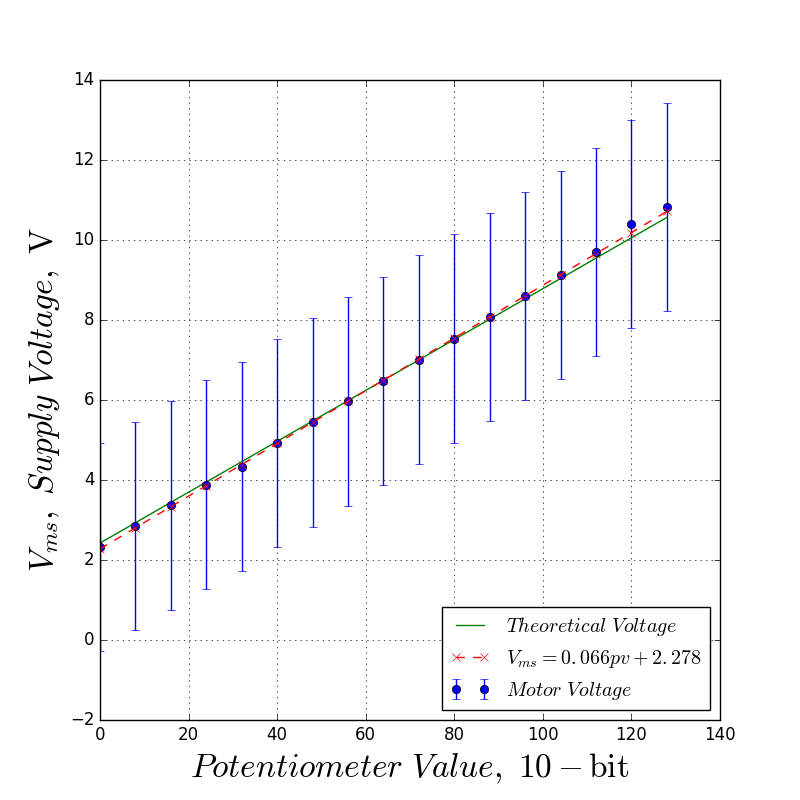
\includegraphics[scale=0.3]{figures/fig_supplyvolt_v_val.png}
				\caption{Motor Supply Voltage vs. Potentiometer Value}
				\label{figvoltvval}
			\end{subfigure}
			\begin{subfigure}[t]{0.45\textwidth}
				\centering
				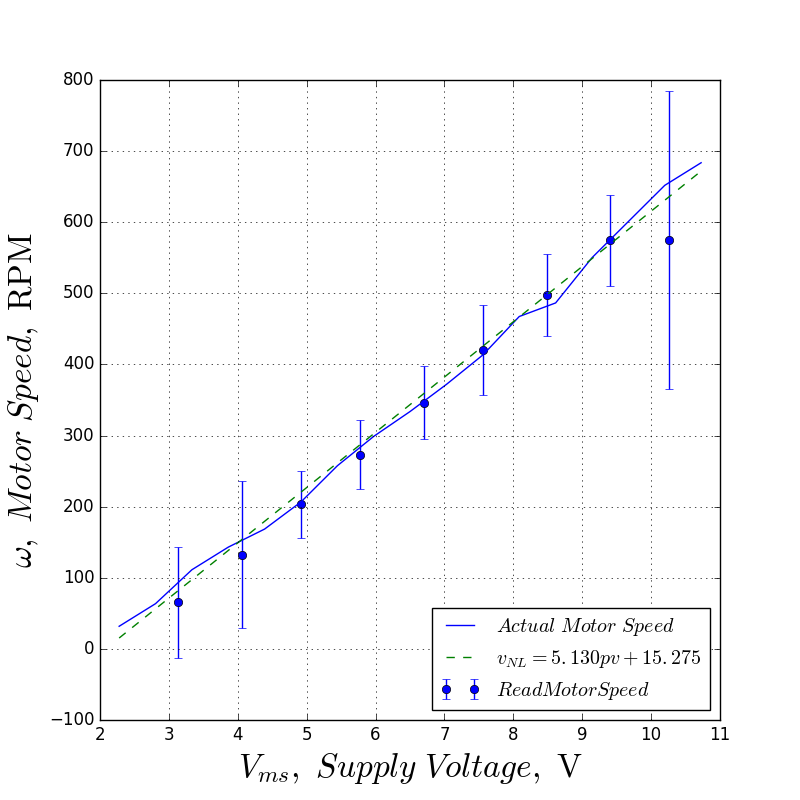
\includegraphics[scale=0.3]{figures/fig_speed_v_val.png}
				\caption{Read Speed and Actual Speed Comparison}
				\label{figdynocheck}
			\end{subfigure}
			%\fbox{\includegraphics[scale=0.25]{figures/fig_shear_behav.png}}
		}
		\label{figspeecal}
		\caption{Speed/Voltage Calibration}
	\end{figure} \newline  \noindent
%	\begin{figure}[!htb]
%		\centering
%		\fbox{\includegraphics[scale=0.3]{figures/figvoltvval.png}}
%		\caption{Motor Voltage Supply vs. Potentiometer Value}
%		\label{figvoltvval}
%	\end{figure} \newline  \noindent

	\subsection*{Speed Measurement} % last edited 14/3/2017
	The rotational speed of the motor needed to be measured accurately and quickly, to be able to calculate the viscosity, and to ensure high enough sample rate that the jamming phenomenon can be seen. This was achieved by using a second motor as a dynamo, linked to the controlled motor via a belt. The dynamo will be spun and generate a voltage proportional to the rate at which it is spun, similar to the speedometer in a car. The magnitude of the voltage can be read in using an ADC by the Raspberry Pi (up to 200,000 samples per second). Accuracy of the set-up was tested using both a slow-motion camera to film the rotation and gauge the actual rotational speed, and a tachometer reading the speed, compared with the value obtained using the dynamo (see Figure \ref{figdynocheck} for results). \br
	Figure \ref{figdynocheck} shows how the actual speed of the motor and the read value compare. It can be seen that the two values correspond well. This uses little of the computing power of the Raspberry Pi as all it has to do to obtain the rotational rate is read a value in from an ADC and perform a simple multiplication; thus this can be performed accurately and at high frequency - well suited to the required purposes.\br
	In order to confirm the accuracy of readings, several videos were taken (at 120fps). The speed was set at a constant value for 10 second periods before filming. Then, every 10 seconds, the potentiometer value is reduced by 8. A mark was made on the rotating cylinder and as this mark passed a certain point, a counter was increased. After the 10 second period, the counter total represented the number of rotations in 10 seconds, the speed in RPM can be calculated by multiplying by 6. This was repeated several times with several different recordings to ensure the resulting correlation was correct.
	%To decipher whether this method was quick enough, the motor was set at a single speed, and the speed was recorded at different set intervals. The standard deviation of the resulting speed curves was taken for each interval. Ideally, these should all be the same and equal to zero. %WHAT?
	
	\subsection*{Speed Calibration} % Rework
	There are several parameters that need to be calculated before the motor can be used in the rheometer. The torque and efficiency characteristic curves of the motor need to be calculated (OR FOUND??). To find this, the digital potentiometer was set to 0 and initial readings of the speed and voltage were taken. Then the value was incremented, the motor speed and voltage were recorded. This was done for every possible value for the digital potentiometer. Using the recorded information, a relationship was found between efficiency and speed. This allows the torque to be calculated using only the electrical power input to the motor, and the rotational speed of the motor (see Equation \ref{eqntorque}).
	\begin{equation}
	\tau = \frac{I \times V \times \eta}{\omega}
	\label{eqntorque}
	\end{equation}
	
	\subsection*{Current Sensor}
	To sense the current drawn by the motor, a hall effect sensor is used. A hall effect is able to produce a voltage proportional to the strength of a magnetic field, a magnetic field which can be produced by running a current through a coil with a magnetically permeable core. The sensor package contains both the coil and the hall effect sensor such that when a current is passed between the sensor pins, a voltage proportional to this current is produced accross the output pins. The sensor used is the ACS712 package using a 5v supply from the Raspberry Pi. The normal output (at zero amps sensed) is half of the supply voltage. The direction of the current will determine whether the current will increase (reverse direction) or decrease (forward direction) this voltage. \br
	The current draw by the motor will only ever be in a single direction, so the direction information is not necessary. To increase the resolution, 2.5v is subtracted from the signal before it is amplified by 10 and fed into the ADC (channel \#1). \br
	The sensor was calibrated by reading in from the sensor and comparing this value with the actual current reading obtained using a standard lab multimeter, repeating this at different voltages (thus also different rotational speeds and different currents). \br
	\cbh %[RESULTS AND SUCH]
	


%=====------++++++=====------++++++=====------++++++=====------++++++=====------++++++=====------++++++=====------++++++=====------++++++=====------++++++=====------++++++=====------++++++=====------++++++=====------++++++=====------++++++=====------++++++=====------++++++

	\chapter*{Conclusions}
	\addcontentsline{toc}{chapter}{Conclusions}
	\def\achapter{Conclusions}
	%Summarise findings and inferences mentioned in the core of the report. Try to be as brief as possible, with concise statements. Include recommendations, where appropriate. 
	
%=====------++++++=====------++++++=====------++++++=====------++++++=====------++++++=====------++++++=====------++++++=====------++++++=====------++++++=====------++++++=====------++++++=====------++++++=====------++++++=====------++++++=====------++++++=====------++++++


	\chapter*{Review}
	\addcontentsline{toc}{chapter}{Review}
	\def\achapter{Review}
	%lit review, history
	%Relate this section to the learning objectives in the introduction. Report what you have learnt about the organisation and about yourself. Mention your achievements, what you have learnt, skills you have acquired or improved. This might be technical or "soft" skills. Try to relate this to what you have learned in your coursework at University and what skills you will take forward to your first full time professional post.
	

%=====------++++++=====------++++++=====------++++++=====------++++++=====------++++++=====------++++++=====------++++++=====------++++++=====------++++++=====------++++++=====------++++++=====------++++++=====------++++++=====------++++++=====------++++++=====------++++++
	\newpage
	\addcontentsline{toc}{chapter}{Nomenclature}
	\def\achapter{Nomenclature}
	%List all the symbols in alphabetical order, with Greek symbols at the end
	\printnomenclature[1.5cm]
	
%=====------++++++=====------++++++=====------++++++=====------++++++=====------++++++=====------++++++=====------++++++=====------++++++=====------++++++=====------++++++=====------++++++=====------++++++=====------++++++=====------++++++=====------++++++=====------++++++
	%Main Bibliography
	\newpage
	\addcontentsline{toc}{chapter}{Bibliography}
	\def\achapter{Bibliography}
	\bibliography{biblio}
	\bibliographystyle{unsrt}
	%\bibliographystyle{apalike}

%% APPENDIX %%


\appendix


\chapter*{Appendices}
\addcontentsline{toc}{chapter}{Appendices}
\def\achapter{Appendices}
\pagenumbering{alph}
\setcounter{page}{1}
\setcounter{section}{1}

\section{1 - Source Code} \label{apxsrc}
As mentioned previously, the software was split up into different sections. This was to make the code more manageable, and easier to debug. The source code for each class section, as well as the filtering library, is included here.
\subsection*{A - ADC}
\begin{verbatim}
INSERT_FROM("./../lib/adc.py")
\end{verbatim}
\subsection*{B - Digital Potentiometer}
\begin{verbatim}
INSERT_FROM("./../lib/dig_pot.py")
\end{verbatim}
\subsection*{C - Motor}
\begin{verbatim}
INSERT_FROM("./../lib/motor.py")
\end{verbatim}
\subsection*{D - Control}
\begin{verbatim}
INSERT_FROM("./../lib/control.py")
\end{verbatim}
\subsection*{E - Filtering}
\begin{verbatim}
INSERT_FROM("./../lib/filter.py")
\end{verbatim}
\section{2 - Design Process Discussion}
\subsection*{A - Voltage Control}
\subsection*{B - Measuring Speed}
The rotational speed of the motor needed to be able to be measured both accurately and frequently (at least 40 times every second - data gathered at most every 25ms). The final design used to meet this specification made use of a dynamo linked up to the motor to gauge the speed of rotation (see Description of Work, page \pageref{chap:dow}). Discussed here are two methods which were considered for use, but were not able to meet the specification.\br 
The first design prototyped for use as a speed sensor was a Hall Effect Sensor coupled with a magnet. The set up was such that every rotation, the magnet would trigger the hall effect sensor and the \rpi would see this trigger as a new revolution. By recording the time between revolution triggers, it would be possible to calculate the rotational speed of the motor. The design was tested for compliance by altering the potentiometer value, thus varying the supply voltage and rotational speed of the motor. The rotations were read in by the sensor, the time of each detection was logged, along with a running log of the speed (recorded every 0.1s). The potentiometer value was held for 10 seconds to allow any dynamic responses in the speed to settle away. If there are any dynamic elements to the motor's speed as a result of a change in voltage, it would show in the results as an altered initial value after a change, which quickly settles to a constant value after  a period of time. The data recorded was evaluated using a histogram plot of the interval times between detected rotations, and a line plot of the measured speed (using both methods) against potentiometer value. \newline \newline \noindent
The histogram should be a single straight line indicating no variation in interval time. If there is found to be small variation in the time, this could be small variation in the supply voltage due to changes in the electrical mains - this would be the main disturbance the control system is working to defend against. Small variation can also be explained away as a leftover between potentiometer value changes with little to no impact on the overall data. Large variation in interval time indicates that something is not right, either with the circuit or the software. It is more likely to be a software error or a limitation of the Raspberry Pi itself rather than a circuit design issue due to the digital nature of the sensor - it can only be on or off. It is unlikely that the sensor is giving a false positive part way through a revolution, or a false negative. \newline \newline \noindent
The line graph of speed against potentiometer value should display two lines which are almost exact copies of each other and are easy to describe lines, preferably linear.\br
	\begin{figure}[!htb]
		\centering
		\fbox{
		\begin{subfigure}[t]{0.45\textwidth}
			\centering
			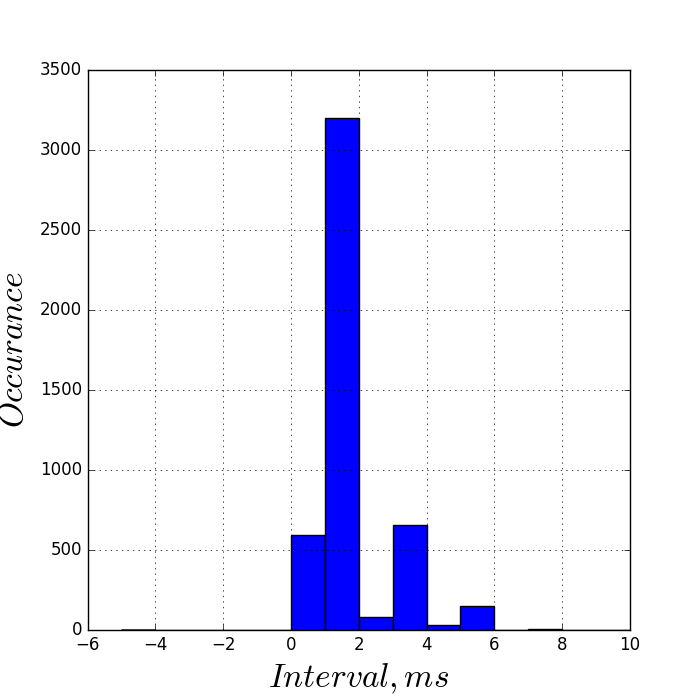
\includegraphics[scale=0.35]{figures/fig_hes_histo.png}
			\caption{Histogram Plot of \newline Sensor Input Interval Time}
			\label{figsenshisto}
		\end{subfigure}
		\begin{subfigure}[t]{0.45\textwidth}
			\centering
			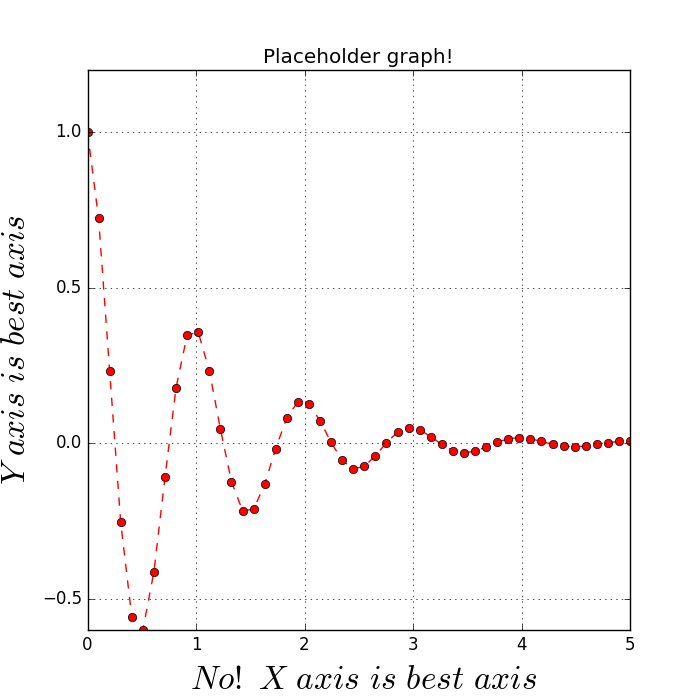
\includegraphics[scale=0.35]{figures/placeholderfig.png}
			\caption{Motor Rotational Speed vs. \newline Digital Potentiometer Value}
			\label{figspeedvval}
		\end{subfigure}
		}
		\label{fig2speeds}
		\caption{Speed Calibration Results}
	\end{figure} \newline  \noindent
	The histogram shows that the intervals are not a constant value (Figure \ref{figsenshisto}). The interval variance is not negligible, and by inspecting the raw data, it was found that the sensor was failing to record some rotations (especially noticable at low speeds). After multiple attempts (with different magnet position, different strengths of magnets) the sensor could not be found to work accurately enough. Perhaps there was a fault in the software, perhaps the \rpi was not able to process the information fast enough, or perhaps the hall effect sensor was simply not able to cope with the repeated switching. The second is highly unlikely; the CPU load on the \rpi was checked on several occasions and was found to only be around 3\% of maximum - the Pi was not at all struggling to run the script.\br
	The speed comparison was [RESULTS2] (Figure \ref{figspeedvval}) therefore this design meets the specified requirements and is suitable for use.
\section{3 - Alternative Designs}
\subsection*{A - Motor Rotation Rate Measuring}
\large Hall Effect Sensor \normalsize \br
A Hall Effect Sensor (HES) is a device which reacts to the presence of a magnetic field. There exist packages containing HESs which can be used to detect the presence of a magnetic field and thus output a digital signal based upon this. The rotational speed of the motor could be detected by attaching a magnet to the rotating cylinder and using an HES (model number US5881) to detect when a magnet passes a point. Using this, the time between the magnet detections can be used to calculate the rotation rate of the motor. \br
The Hall Effect Sensor is powered by the Raspberry Pi's 5v line and connected to ground. The output pin will be in a high state (0.6v) until the sensor detects the south pole of a magnet, at which point the output will go low (0v). To communicate with the Raspberry Pi, this signal must be converted into 3.3v logic (either a 3.3v high signal or 0v low signal). To achieve this, GPIO pin 23 on the Raspberry Pi was pulled high (set to a high logic signal) and connected through a transistor to ground. Normally, the high input to the transistor allows the flow of current from the GPIO pin to ground, meaning it has a low value. When the hall effect sensor detects a magnet the high signal to the transistor will block the flow of current between the GPIO pin and ground - the GPIO pin will go high. Figure \ref{circhall} shows the schematic of this circuit. \newline
\begin{figure}[!htb]
	\centering
	\fbox{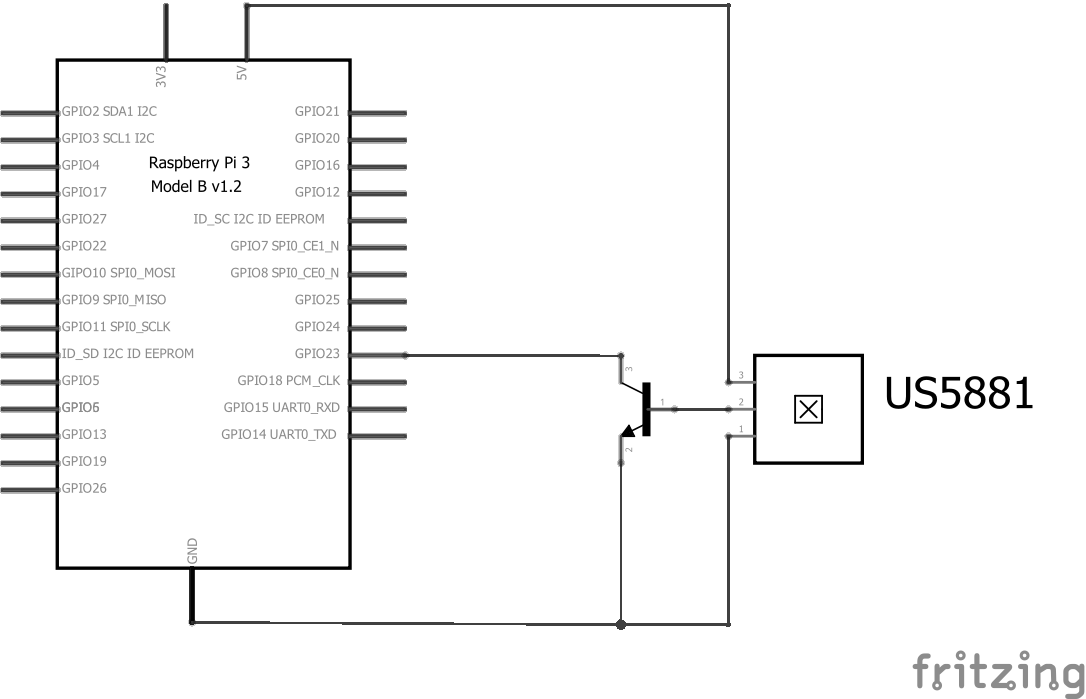
\includegraphics[scale=0.3]{images/circspeeddet.png}}
	\caption{Hall Effect Speed Detector Circuit Diagram}
	\label{circhall}
\end{figure} \newline  \noindent
This circuit does not measure the instantaneous rotational speed of the motor. Instead it measures the average speed. By using more magnets, and a smaller time-frame, the speed measured becomes closer to an instantaneous speed. The advantage of using this circuit is that it is simple to set up and use, other speed detection circuits require the use of lasers and photodiodes/phototransistors, or dc dynamos and analogue to digital converters. However, the main downside lies in having to attach magnets at regular intervals to the rotating cylinder, which will have to be done accurately. Another downside is the range of the hall effect sensor. The sensor must be within 10mm of the magnet for it to be able recognise it. \newline \newline \noindent
\large Light Sensor \normalsize \br
The rotational speed of the motor was measured using a light-gate type set up. An IR-LED and IR-phototransistor were set up near the inner cylinder. A metal trip was attached to the cylinder such that it broke the light beam between the LED and the phototransistor. The transistor was set up as a switch such that when light was allowed to fall onto the transistor, a complete circuit was made between GPIO23 (pulled high by the build in resistor) and ground on the Raspberry pi, thus a low value is read. When the beam is broken, this circuit breaks too, causing the value of GPIO23 to go high. On the software side, this value change can be detected and the timing of which can be used to calculate the speed. \newline
\section{4 - Further Information}
\subsection*{A -  Programming Languages}
Programming languages come in many forms. High level languages (like C, Java, C\#, Python) are abstracted from the binary in which it will be eventually stored. High level languages consist of a natural-like language which is converted by a "compiler" or "interpreter" into machine code, understandable by the processor \cite{proglanghighlow}. \br
\noindent
An example of a high level language (Python):

\begin{verbatim}
        import time                                   # using the "time" package
        
        while True:                                   # loop the following forever:
            print time.strftime("%X", time.gmtime())  # print the current time (HH:MM:SS)
\end{verbatim}
An example of a machine code (in hexadecimal)\cite{proglangmachex}:
\begin{verbatim}
            0x 60 00 00 80
            0x A4 00 00 00
            0x 60 01 00 84
            0x A4 01 01 00
            0x 60 02 00 00
            0x 60 03 00 04
            0x 60 04 00 00
            0x 60 05 00 01
            0x 08 00 00 02
            0x 20 00 00 03
            0x 20 04 04 05
            0x 11 20 04 01
\end{verbatim}
From the above it can be seen that high level languages, while not strictly English, are far easier to read than machine code. Machine code will take multiple instructions to achieve the same thing that could be done in a single line in a high level language, thus a high level instruction needs to be converted into multiple machine level instructions for the processor to understand it. There are different ways of doing this, leading to diversity in the types of high level languages. \hi (MISSING LINK) \nohi. Object Oriented Programming Languages (OOPLs) deal with data in terms of "objects"\cite{proglangwhatisoopl}. An object is, like the name suggest, something. This something has properties, and can have things done to it. In the above Python example, "alarm\_time" is a number object, and it is being assigned a value. A "method" is a way of doing something in the program. In the above, the "time()" method is used to get the current time (in number of seconds since 1 January 1970). The advantage of OOPLs lies in the ability to collect objects and methods together in a class. The "time" class above contains a lot of methods which can be used by the programmer, in the example the "time.time()" method is called from the class. The programmer can therefore define a set of methods for dealing with some data in a certain way in a class, and then create multiple instances of this class with different starting data to make use of different starting data. For example, a "sphere" class could be written, with methods which provide the sphere's surface area and volume, given the sphere's diameter. Then a program could be written to create three sphere class instances, each with different diameters and then the areas and volumes could be calculate simply when needed. This creates tidy programs, which are easier to understand and reduces the amount of redundant code that needs to be written. \br
Another, less common, type of programming language is the procedural language. This language is simply one instruction following another\cite{proglangwhatisoopl}. The procedural program starts at the start and continues down the list of instructions until it finishes. This language requires writing out the same code multiple times to achieve the same effect as an OOPL, which is a reason for its reduced popularity. \br
As previously mentioned, code written in a programming language is usually compiled before it is run. However, some languages do not need to be compiled before being run. These languages are called "interpreted" languages and they are "compiled" line by line when you run them \cite{proglanginterp}. Since interpreted languages do not need to be compiled (and so software developers do not have to wait for the compilation step to complete before testing) they are preferred for developing software. However, they tend to run slower than compiled programs for the same reason. \br
To conclude this section,  programming languages are varied and have different advantages and disadvantages. The correct programming language must be chosen for the correct situation.

\subsection*{B -  Signal Noise Reduction}
Analogue readings of real world data can be corrupted by noise. Noise can appear due to fluctuations in atmospheric conditions, electrical supply, or thermodynamic fluctuation in the reading material (to name a few). For the data to be useful, there must be some provision for reducing the noise. Signal filters can be used to reduce the amount of noise, these can be hardware or software filters. Both represent the same concepts, but in different implementations. Hardware implementation is in continuous time, while software uses discrete time approximations of the same models and functions as hardare filtering. Discussed here are software filtering techniques. \br

% notes -->>
% transform based signal processing methods
%	"express a signal in terms of a combination of a set of elementary signals [... that can be easily analysed]"
% source-filter model based signal processing
%	use a model to obtain the true form of the signal - expressing the predictable structures of the signal, expected patterns.
%	sensitive to deviations from the model
%	used in voice recognition, telephony, video encoding, high-res spectral analysis
% bayesian statistical model based signal processing
%	uses cost-weighted (bayesian philosophical) probability to obtain a model of the "statistical average" values
% neural networks XX
% <<-- notes from wileyadvsignproc.pdf

% from messing around, butterworth seems to give the best representation of the data as noiselessly and as correct as possible.
\begin{figure}[!htb]
	{\centering
	\fbox{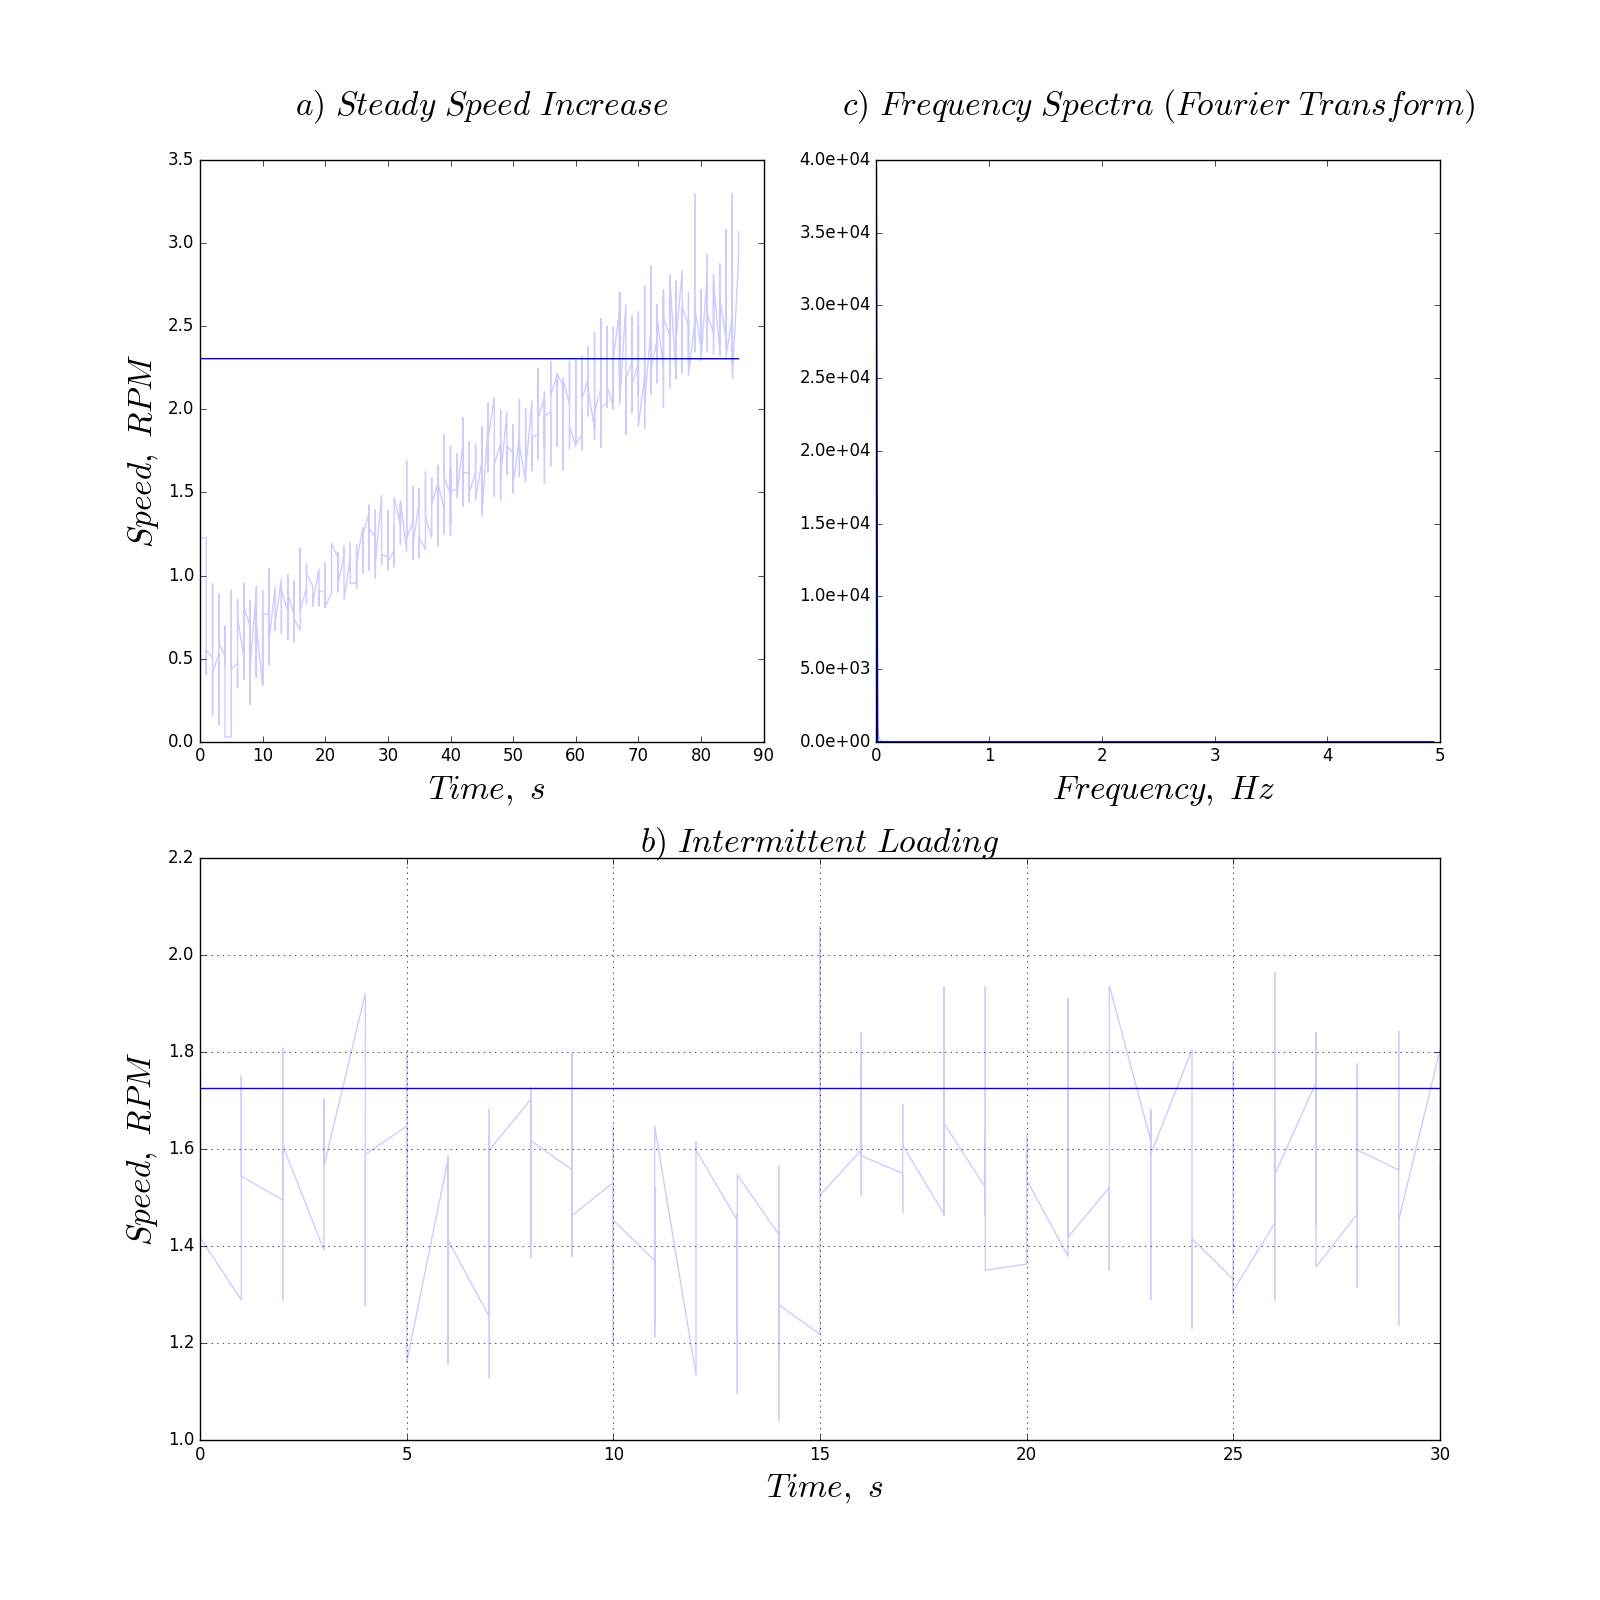
\includegraphics[scale=0.35]{figures/fig_filt_demonstra.png}}
	\caption{Butterworth Filter Demonstration}
	\label{figfilterdemon}}
	%optional:
	{\footnotesize Actual data readings (faint blue) were passed through a Butterworth filter to obtain a noise-reduced signal (bright blue).\newline {\bfseries a)} Graph of a steady increase in motor supply voltage, excpeted result is a series of 11 steps.\newline {\bfseries b)} Graph showing speed variance with a random intermittent load applied to the motor (an approximation of a shear thickening fluid)\newline {\bfseries c)} Fourier Transform of the response in b); faint blue line shows the fourier transform of the raw (noisy) data, birght blue shows the filtered response, clearly showing the effect of the filter on the resulting data.}
\end{figure}
%Appendix Bibliography

\end{document}